\chapter{Developing a Framework for Classification}

The volume of data and complexity pose a significant challenge when developing methods to identify and classify emission-line stars. These and other constraints indicated that it would not be efficient or an effective use of time to trial multiple machine learning methods in pursuit of the end goals. Instead, this work developed a general framework and set of principles based on the background provided in Chapters 1 to 3. These principles guided the development of a viable prototype method upon which the total machine learning method was built. The details of this framework, the methods that were selected as well as the raison d'être for these decisions and the results from the prototype are presented in the following sections.

\section{Requirements and Constraints}

It was demonstrated in prior chapters that morphological classification based on naked eye observations of spectra cannot scale with the volume of data present in GALAH DR3. And while machine learning methods such as t-SNE and autoencoders \citep{traven2017galah, vcotar2021galah} have been relatively successful in detecting H$\upalpha$ emission spectra, they are both unable to further classify emission-line spectra into classes such as P Cygni and inverse P Cygni.

When developing a framework for classification, this work found that an approach that is sensitive to the meaningful morphological differences between P Cygni, inverse P Cygni and other species is an important requirement. Feature engineering must capture the understanding that P Cygni spectra exhibit a red shifted emission peak while the inverse P Cygni spectra exhibit a blue shifted peak and must be able to differentiate between classes such as double-peaked emission spectra and emission lines superimposed on absorption. This can be quite intuitive for a human being to do manually but can prove challenging for a machine. Finally, given that the feature space is of size $\sim$ \num[round-precision=2,round-mode=figures, scientific-notation=true]{2928752091}, a classification method must be able to overcome the "curse of dimensionality" and be computationally and memory efficient.

Given that DR3 does not have labeled samples of P Cygni and inverse P Cygni spectra, a supervised learning approach to classification was not suitable. This narrowed the approach to the unsupervised learning domain \citep{hastie2009elements}. Chapter 2 demonstrated that well known unsupervised clustering methods such as k-means clustering failed to cluster and classify emission-line spectra \citep{garcia2018machine}, this work did not consider this and related methods. Instead, this work took a first principles based approach, with a focus on methods that are sensitive to morphological similarities and differences between spectra. More rudimentary methods such as cross-correlation of signals are examples of methods that could be sensitive to the various emission line morphologies. However, given that a labeled data set of the various classes of emission-line spectra in DR3 did not exist, this line of inquiry was abandoned as this work was unable to create mean spectra capable of convolving against all DR3 spectra for the various potential classes. Instead, this work explored methods that created effects similar to pairwise cross correlation, provided a similarity score (or equivalent) with limited human intervention and with minimum reliance on rule based approaches that have been used in the past \citep{traven2015gaia}. 

These constraints allowed this work to narrow the search for suitable methods to a field known as unsupervised time series clustering, more specifically a clustering method based on a concept used extensively in signal processing called dynamic time warping (DTW) \citep{kruskal1983overview}. First introduced in 1975 as an algorithm for speech recognition \citep{itakura1975minimum}, DTW has been modified and adapted extensively in various scientific disciplines such as signal processing, telecommunications and biomedical engineering. It was demonstrated in Chapter 2 that DR3 spectra and indeed all spectra are mathematically analogous to time series. While an individual spectrum does not contain a time axis, the monotonically increasing wavelength grid serves as the analogue of the time axis. Time series methods such as DTW have been more generally developed in the domain of time series analysis \citep{nielsen2019practical} and can be suitably adapted to stellar spectra. With clustering, this work did not rely on labelled data, it rather took a data-driven approach that learns from the emission-line morphologies present in the normalised spectral data present in DR3.

\section{Dynamic Time Warping}

Dynamic time warping (DTW) is a time series analysis algorithm that can measure similarity between two temporal sequences. The similarity can then be used to cluster morphologically similar spectra into meaningful groups. These clusters can then be used to classify spectra into distinct classes. 

DTW is suitable for clustering problems where the morphology of the signal plays a salient role over other features \citep{nielsen2019practical} and where labeled data is unavailable. The name is inspired by the method itself where two signals are stretched or warped to align them on the temporal axis. For stellar spectra, this warping takes place in the wavelength domain and thus produces a discrete dynamic wavelength warping effect.

\begin{figure}[!htb]
\centering
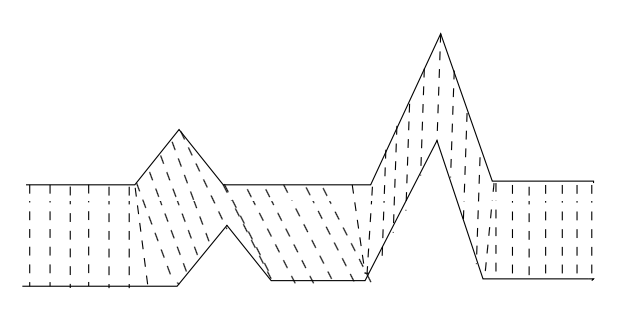
\includegraphics[scale=1]{figures/Dynamic_time_warping.png}
\caption{Each point on the wavelength grid is mapped to a point on the opposite spectrum, but there is no requirement that the mapping is one to one. Reproduced from Nielsen \citep{nielsen2019practical}}
\label{fig4.1}
\end{figure}

As indicated in Figure \ref{fig4.1} above, the algorithm works by expanding or contracting the wavelength axis to find the best alignment and thus ensuring that morphologically similar spectra can be compared. This algorithm is often described as being similar to comparing the shape of signals visually. The algorithm follows several steps and constraints which are as follows,

\begin{enumerate}
    \item Every point on the spectrum must be matched with at least one point of the other spectrum
    \item The first and last indices of each spectrum must be matched with their counterparts in the other spectrum
    \item The mapping must be such that the wavelength is increasing rather than decreasing i.e. the method should not match a point on on spectrum to a point on the other spectrum that has passed. 
\end{enumerate}

Steps 2 and 3 do not have a significant impact on the data set being used in this work as the data is sampled to the same wavelength grid and are thus of equal length. 
There are many possible ways to align two spectra while adhering to these constraints. The algorithm chooses the alignment that minimises the distance between the spectra. This distance is a cost function and is measured as the sum of the absolute differences between matched points. The absolute difference in this context is the difference between the points' values (wavelength values). This work relies on this distance measure to serve as the basis for clustering.


The Pythonic representation of this algorithm is as follows,

\begin{lstlisting}[language=Python]
# Primary function
def distDTW(lambda1, lambda2):
     DTW={}
     for i in range(len(lambda1)):
         DTW[(i, -1)] = np.inf
     for i in range(len(lambda2)):
         DTW[(-1, i)] = np.inf
     DTW[(-1, -1)] = 0
 
# Calculate the optimum i.e. where distance is minimum
     for i in range(len(lambda1)):
         for j in range(len(lambda2)):
             dist = (lambda1[i] - lambda2[j])**2
             DTW[(i, j)] = dist + min(DTW[(i-1, j)],
                                      DTW[(i, j-1)], 
                                      DTW[(i-1, j-1)])
 
 # Return the associated distance between two spectra
     return sqrt(DTW[len(lambda1)-1, len(lambda2)-1])
\end{lstlisting}

Despite the effectiveness of this algorithm, the computational complexity is of order $O(N^2)$. As this presents a significant computational cost and overhead, this work relies on a linear time complexity i.e. the $O(N)$ Python language implementation of DTW called \texttt{FastDTW} to compute the optimum distance between spectra and thus the similarity \citep{salvador2007toward}. \texttt{FastDTW} is a linear approximation to the DTW method above. A full discussion of how it compares to other implementations of DTW is beyond the scope of this thesis. 

In addition to computational complexity, an important consideration is available memory. Generally, all spectral data must be loaded into memory (RAM) when computing DTW distances. In the case of DR3, this implies holding $\sim$ \num[round-precision=2,round-mode=figures, scientific-notation=true]{2928752091} features in memory. The computational hardware available for this project had a memory capacity of $\sim$ 300 GB. \texttt{FastDTW} in particular required a memory capacity of at least 1TB for the $\sim$ \num[round-precision=2,round-mode=figures, scientific-notation=true]{2928752091} features. This is a significant amount of data to hold in memory and presented a challenge.

This work presents two strategies to overcome these challenges and reduce computational and memory overheads. These are as follows,

\begin{enumerate}
    \item Reduce the number of features. As explained in a Chapter 2, this work pre-selects only the region around H$\upalpha$. \texttt{FastDTW} was run on this region only.
    \item Reduce the search space from the entire DR3 data set to a subset which has a higher chance of yielding P Cygni, inverse P Cygni and other emission-line spectra - The existence of H$\upalpha$ emission-line spectra is a precursor to the existence of P Cygni and inverse P Cygni spectra Thus this work used the H$\upalpha$ emission-line data set from Čotar et al.\citep{vcotar2021galah} for prototyping this method. This subset with $\sim$ 10,000 spectra includes data from both GALAH and other related surveys. Presumably, this data set only contains H$\upalpha$ emission-line spectra and not typical spectra.
\end{enumerate}

There are many machine learning methods that can be used to cluster groups of similar and dissimilar observations. These methods will generally compute method specific distances measures as a similarity metric. DBSCAN for example computes a method specific distance which cannot be overridden by a pre-computed distance metric such as a DTW distance \citep{traven2017galah}. It is unclear whether a DBSCAN distance metric, or indeed a distance metric other than DTW can capture the morphological features of emission-line stars. Due to time constrains, this work did not evaluate the alternative distance metrics provided by the various clustering methods that are open to the researcher. Instead, this work chose a clustering method which can accommodate pre-computed distances such as a DTW distance. Agglomerative hierarchical clustering is a method that can take a pre-computed distance metric such as a DTW distance, and use it to cluster observations into classes. It is a well understood and robust method that has proven to work well on time series problems that rely on DTW distances \citep{nielsen2019practical}.

\section{Agglomerative Hierarchical Clustering}

With a similarity measure such as the pairwise DTW distances between spectra, hierarchical clustering can be used to group similar spectra into similar clusters. Once a similarity measure (or a dissimilarity measure) has been specified, hierarchical clustering produces a representation in which clusters at each level of the hierarchy are created by merging clusters at the next lower level. At the lowest level, each cluster contains a single observation. At the highest level, there exists a single cluster that contains all of the data \citep{hastie2009elements}. There are two basic paradigms to traverse these levels or tree, namely, aggolomerative (bottom-up) and divisive (top-down). 

With agglomerative clustering, initially, each spectrum will initially form a singleton cluster. At each step, the most similar spectra will be merged into a single cluster, producing one less cluster at the next higher level. The similarity between two spectra is based on the pre-computed DTW distance between them. A lower distance implies a greater similarity while a higher distance indicates a dissimilarity.  

Based on the similarity (and dissimilarity) between individual spectra, a \emph{cluster dissimilarity} can also be defined. Consider two clusters called $A$ and $B$. The dissimilarity between the two clusters $d(A,B)$ is computed from the set of pairwise dissimilarities $d_{ij}$, where one member of the pair $i$ is in $A$ and the other $j$ is in $B$. The \emph{complete linkage dissimilarity} between the two clusters is set to be the dissimilarity of the furthest (most dissimilar) pair of spectra,

\begin{equation}
    d(A,B) = \max_{\substack{i \in A \\ j \in B}} d_{ij}
\end{equation}

This is also known as the farthest neighbour method. Other dissimilarity measures such as \emph{single linkage dissimilarity} or nearest neighbour dissimilarity can be defined as

\begin{equation}
    d(A,B) = \min_{\substack{i \in A \\ j \in B}} d_{ij}
\end{equation}

Hierarchical clusters can be visualised using a dendogram. A dendogram is a binary tree that represents the recursive agglomeration (or division) of clusters. The height of the tree (or a branch) is proportional to the inter-group dissimilarity defined above. 

\begin{figure}[!htb]
\centering
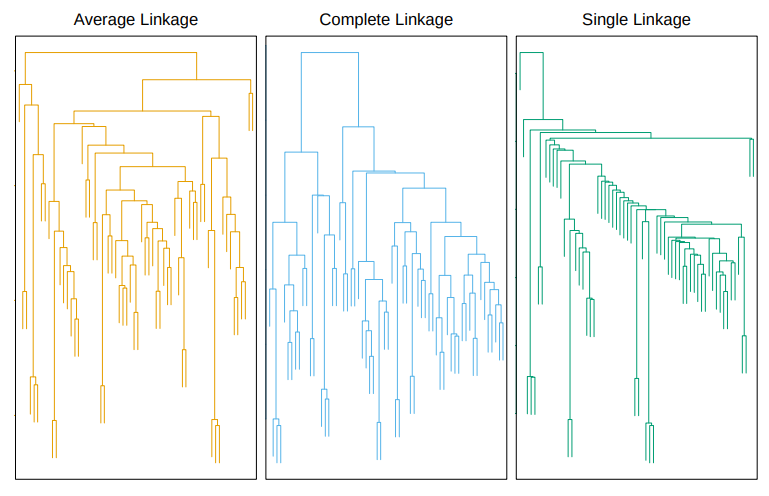
\includegraphics[scale=0.60]{figures/complete linkage.png}
\caption{Dendograms for the same toy data set using different similarity measures. Note the longer branch lengths of the complete linked tree that selects for maximum dissimilarity. Reproduced from Hastie et al. \citep{hastie2009elements}}
\end{figure}

This work used the complete linkage dissimilarity to cluster spectral groups. The justification for using this measure over the single linkage dissimilarity is to force the separation of P Cygni and inverse P Cygni spectra into distinct groups by exploiting the maximum distance between two individual spectra that belong to these groups. Other distance measures such as group average clustering uses the average dissimilarity between the groups. Group average clustering can be less accurate in separating the data into clusters as it relies on an average spectrum per cluster which may not completely capture the variation of spectral morphologies within a cluster. Therefore this work did not consider this measure as it may be less accurate in separating P Cygni from inverse P Cygni and other emission-line spectra due to this averaging or smoothing effect. This work also relies on the agglomerative (bottom-up) method as it is more robust and has been studied extensively in the literature compared to the divisive (to-down) method \citep{hastie2009elements}.

\subsection{Selecting the Number of Clusters}

Given that the framework proposed above is an entirely unsupervised machine learning approach, it is generally not required that the number of clusters be specified in advance. In the absence of a predefined value for this parameter, the typical approach would require a plot of the dendogram where suitable cuts can be made at a required level. However since the tree can theoretically be cut at any level and can have a maximum number of clusters equal to the number of samples and a minimum number of clusters equal to 1, as will be demonstrated below, a more meaningful and reliable cut can be made with the aide of astrophysical domain knowledge. In the absence of such knowledge this work would have to cut the dendogram at each level, the examine the clusters and subsequently decide on a suitable number of clusters. Furthermore, given that the sample size is at least 10,000 spectra, visually inspecting a dendogram for this data set can be challenging. Where possible, this work used prior art such as Reipurth et al. \citep{reipurth1996halpha}, Traven et al. \citep{traven2017galah}, and Zhang et al. \citep{zhang2021catalog} to determine the number of clusters, thus eliminating the requirement to visually inspect a complex dendogram of the order of thousands of branches. 

Classes of H$\upalpha$ emission-line spectra have been found using manual methods and as such prior work can provide some guidance regarding the number of clusters. Reipurth et al. in particular proposed the existence of seven morphological groups which include P Cygni and inverse P Cygni, as well as five other H$\upalpha$ emission-line classes \citep{reipurth1996halpha}. If the number of clusters is set to a value of two, there is a significant risk that other morphologies will be included in the P Cygni cluster and inverse P Cygni cluster thus leading to erroneously classified/labelled clusters. Thus based on the prior art, this work took the number of clusters to be between six and ten as a suitable range. The number of samples were significantly higher than any data sets previous prior art, especially the manual classification approaches detailed in prior chapters. The justification to use a higher number of clusters such as ten is to account for the possibility of additional morphological classes that may have been missed in the prior art during manual classification. As it will be demonstrated in Chapter 6, this over-classification can be beneficial when working with more complex data sets.

\section{Results}

The results of the DTW distance calculation can be visualised as a distance cost plot. Figure \ref{fig4.3} presents the pairwise distances for 6,977 samples from DR3 that are present in the Čotar et al. data set after the application of DTW. Note that the plot resembles a triangular matrix with the diagonal representing a value of zero for the self distance of a spectrum. Lower values indicate higher similarity while higher distance values indicate lower similarity (or greater dissimilarity). Zooming in to a region reveals further structure concerning similar and dissimilar spectra. The self similar, zero distance diagonal and the triangular nature of the distance matrix, are is visible on this plot.

\begin{figure}[!htb]
\centering
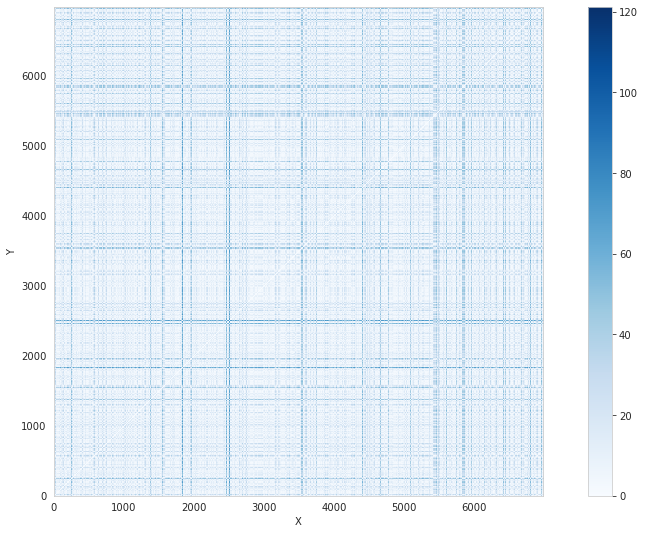
\includegraphics[scale=0.60]{figures/dtw cotar.png}
\caption{Pairwise DTW distances for spectral samples in Čotar et al.}
\label{fig4.3}
\end{figure}

This distance matrix was used as the basis for complete linkage aggolomerative hierarchical clustering. The number of clusters was varied between seven and ten. A mean silhouette score was calculated for each selection. This score was used as an additional selection criterion for the number of clusters. Silhouette scores can range between -1 and 1. Negative scores indicate that samples may be assigned to the wrong cluster. Values extremely close to zero indicate that clusters may overlap. The best achievable value is 1, although this is rarely achieved in practical unsupervised clustering problems of this nature. Thus the silhouette score is a measure of the efficacy of the clustering process.

\begin{figure}[!htb]
\centering
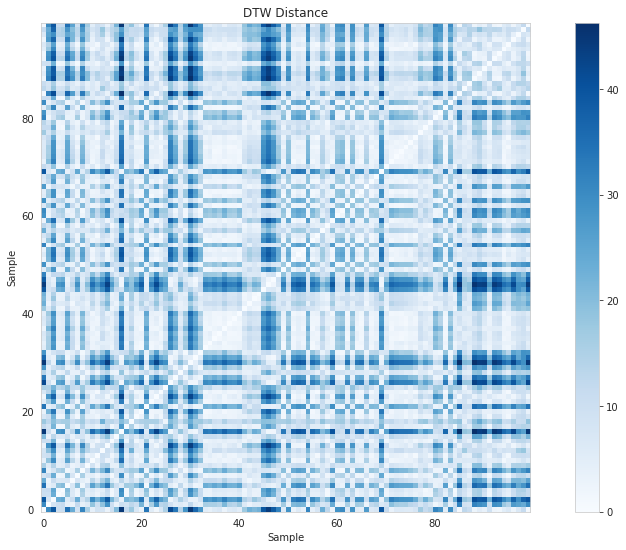
\includegraphics[scale=0.60]{figures/dtw cotar zoomed.png}
\caption{Pairwise DTW distances for spectral samples in Čotar et al. (zoomed).}
\end{figure}

In order to calculate the mean silhouette score, silhouette coefficients for all samples must be calculated as follows. Compute the mean intra-cluster distances given by $a$ and then compute the mean nearest-cluster distance $b$ for each sample. The sample silhouette coefficient is then given by,

\begin{equation}
\frac{(b-a)}{\max_{}(a,b)}
\end{equation}

Once the coefficient for each sample was calculated, the mean silhouette score for the entire sample was computed. Table 4.1 summarises the scores obtained.

\begin{table}[]
\begin{center}
\begin{tabular}{|c|c|}
\hline
\textbf{Number of Clusters} & \textbf{Silhouette Score} \\ \hline
6                     & 0.2904                    \\ \hline
7                     & 0.3033                    \\ \hline
8                     & 0.3005                    \\ \hline
9                     & 0.3092                    \\ \hline
10                    & 0.3044                    \\ \hline
\end{tabular}
\caption{Silhouette score comparison}
\label{table:Silhouette Score}
\end{center}
\end{table}

At face value it appears that nine clusters is the optimum given that this produces the largest silhouette score. However upon closer examination it was concluded that ten was more suitable under the essential constraint that P Cygni and inverse P Cygni spectra should be adequately separated from other clusters. Thus, the spectra that belong to each cluster for both nine clusters and ten clusters were plotted. For nine clusters, while a P Cygni only cluster was identified, a cluster containing inverse P Cygni spectra was not identified. However when this parameter was set to ten, two clear clusters of P Cygni and inverse P Cygni spectra were identified.

\begin{figure}[!htb]
\centering
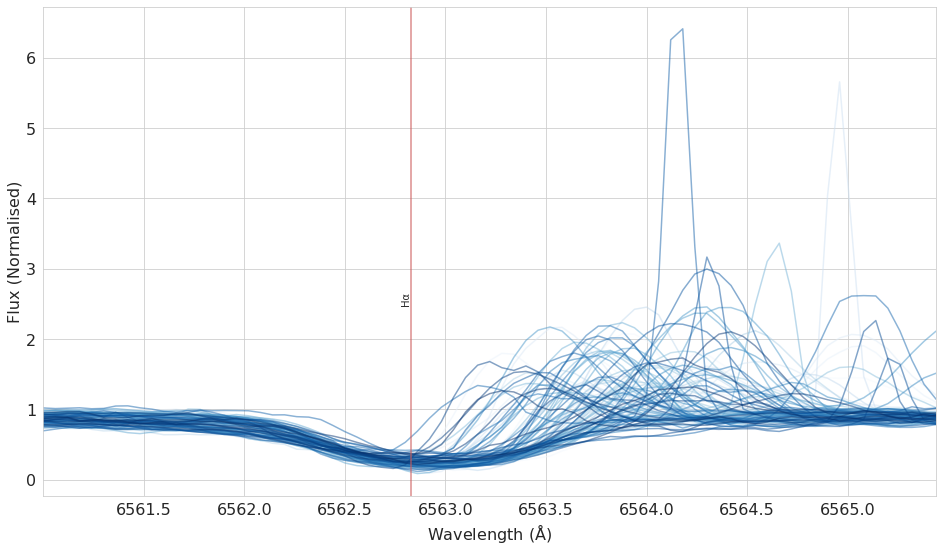
\includegraphics[scale=0.45]{figures/pcygni.png}
\caption{102 P Cygni spectra identified using clustering.}
\end{figure}

\begin{figure}[!htb]
\centering
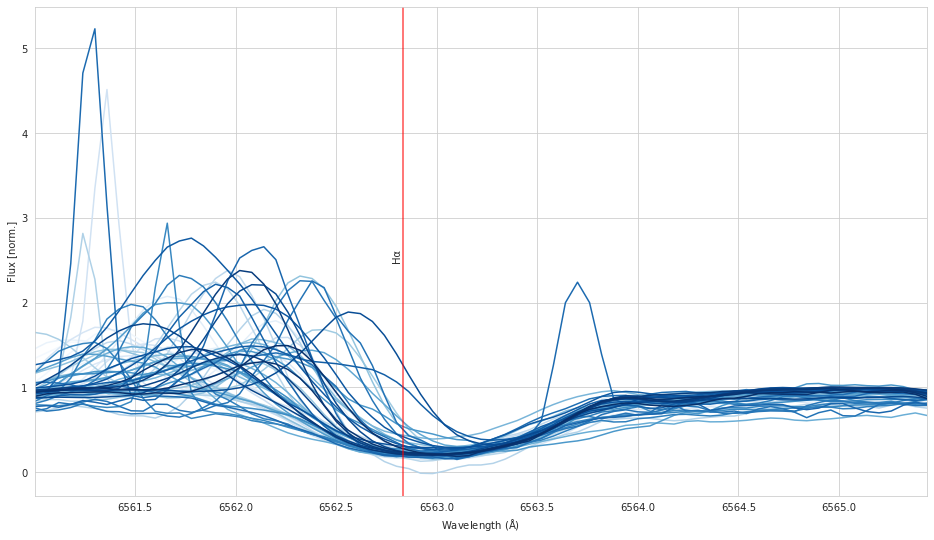
\includegraphics[scale=0.45]{figures/inverse p cygni.png}
\caption{62 Inverse P Cygni spectra identified using clustering.}
\label{fig4.6}
\end{figure}

Eight other clusters with various emission-line morphologies such as double peak were also identified. A full gallery of these classes is presented in the appendix. Given the silhouette score, it is possible that some P Cygni and inverse P Cygni spectra may have been mis-classified (see Figure \ref{fig4.6}) and included in other classes. This can be addressed by further sub-clustering and classification of spectra via a second pass of the scheme above. This work however, did not progress with multiple passes of this method due to time constraints. 

A sub-classification of the P Cygni and inverse P Cygni classes discovered in this process is presented in Chapter 5 where these results are compared to t-SNE. The merits and demerits of this approach compared to t-SNE is discussed further in this chapter. 

\section{Line Fitting}

The P Cygni and inverse P Cygni spectra thus classified were modeled using a double Gaussian with an offset for one of the Gaussian functions \citep{traven2015gaia, traven2017galah, zhang2021catalog}. This mixture model with two Gaussians can be used to fit the line profile of P Cygni and inverse P Cygni spectra. Given that there are 102 P Cygni spectra that require fitting, this work adopted a semi-automated method where the initial conditions for the model parameters were driven by the data. Notably the minimum and maximum local flux values were used to set both the amplitude and mid value of each peak and trough.

This work then utilised the popular Python based numerical optimisation package, \texttt{scipy} \citep{2020SciPy-NMeth} to generate fitted models for the P Cygni and inverse P Cygni spectra using least squares optimisation.

The Gaussian mixture model is defined as, 

\begin{equation}
    f(x) = \frac{A}{\sigma_1\sqrt{2\pi}} 
  \exp\left( -\frac{1}{2}\left(\frac{x-\mu_1}{\sigma_1}\right)^{\!2}\,\right) + \frac{B}{\sigma_2\sqrt{2\pi}} 
  \exp\left( -\frac{1}{2}\left(\frac{x-\mu_2}{\sigma_2}\right)^{\!2}\,\right) + C
\end{equation}


This seven parameter model contains an offset parameter $C$ to account for the inverted Gaussian required to model the absorption trough/line of the P Cygni and inverse P Cygni spectra. The parameters A and B are to account for the respective amplitudes of the emission and absorption lines. The uncertainties of this fit can be modelled more accurately within a Bayesian framework and the use of MCMC estimation \citep{hogg2010data}. However this is beyond the scope of this work.

\begin{figure}[!htb]
\centering
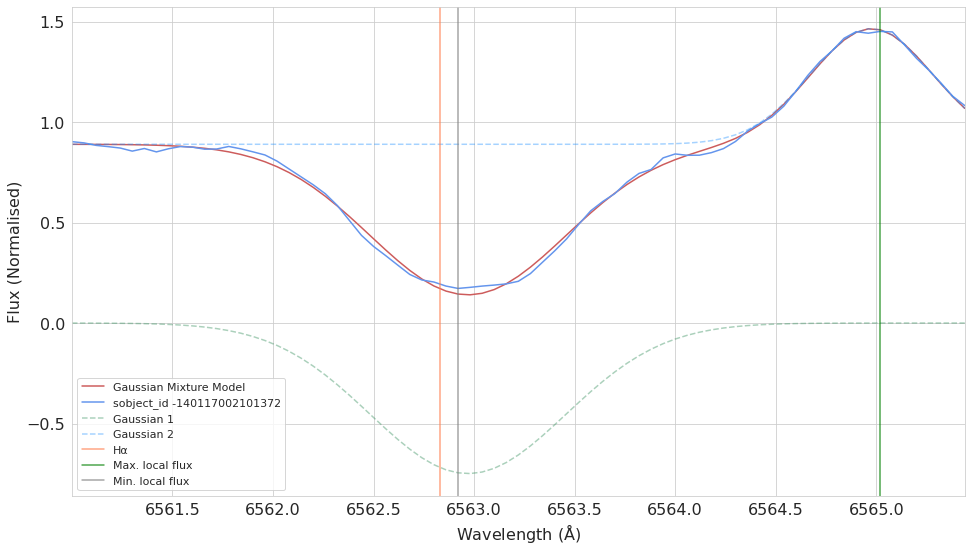
\includegraphics[scale=0.45]{figures/p cugni fitted.png}
\caption{A Gaussian mixture model fit of one of the identified P Cygni spectra.}
\end{figure}

The process can be repeated for each P Cygni spectrum discovered by clustering. Presented below are a few examples of these fitted models. 

\begin{figure}[!htb]
\centering
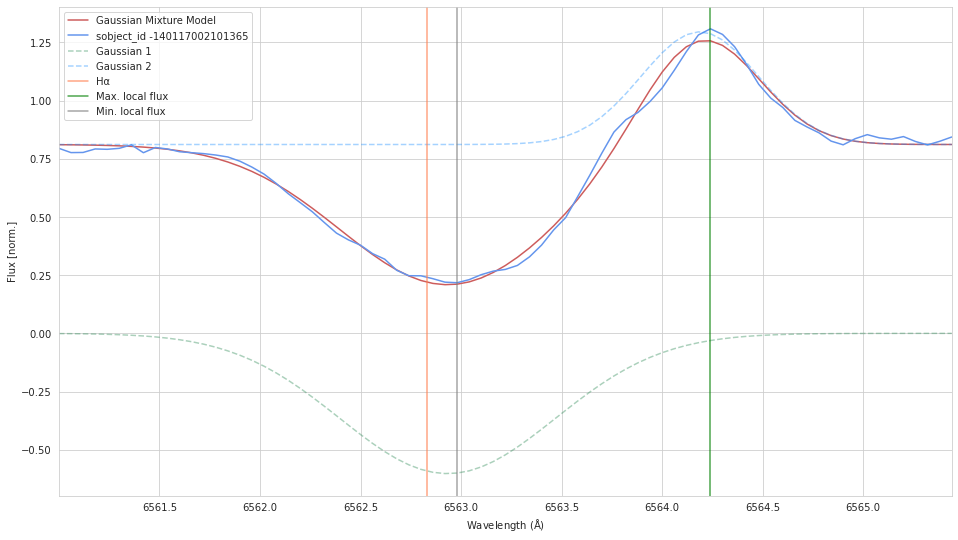
\includegraphics[scale=0.45]{figures/p cygni fitted 2.png}
\caption{A Gaussian mixture model fit for sobject ID 140117002101365. }
\end{figure}

\begin{figure}[!htb]
\centering
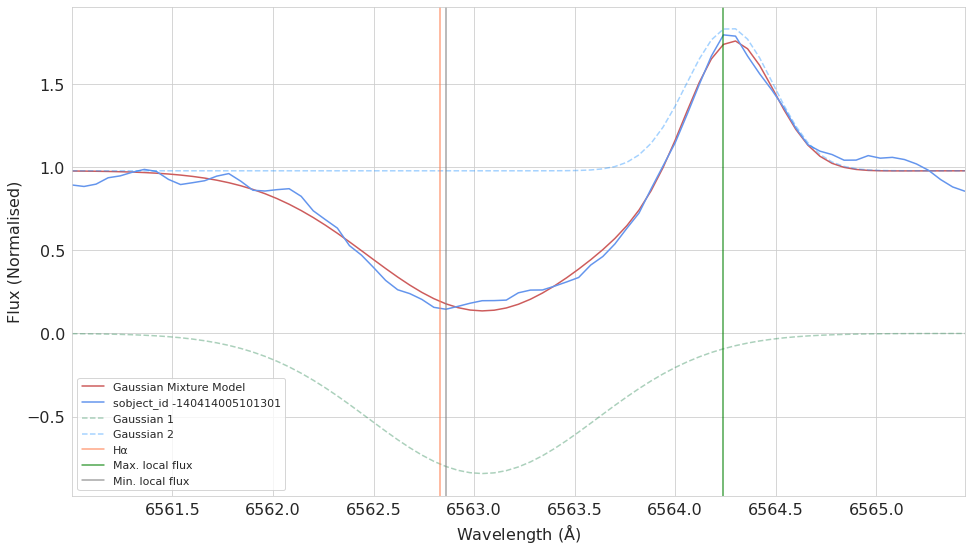
\includegraphics[scale=0.45]{figures/p cygni fitted 3.png}
\caption{A Gaussian mixture model fit for sobject ID 140414005101301. }
\end{figure}

This process was also extended to the inverse P Cygni spectra.

\begin{figure}[!htb]
\centering
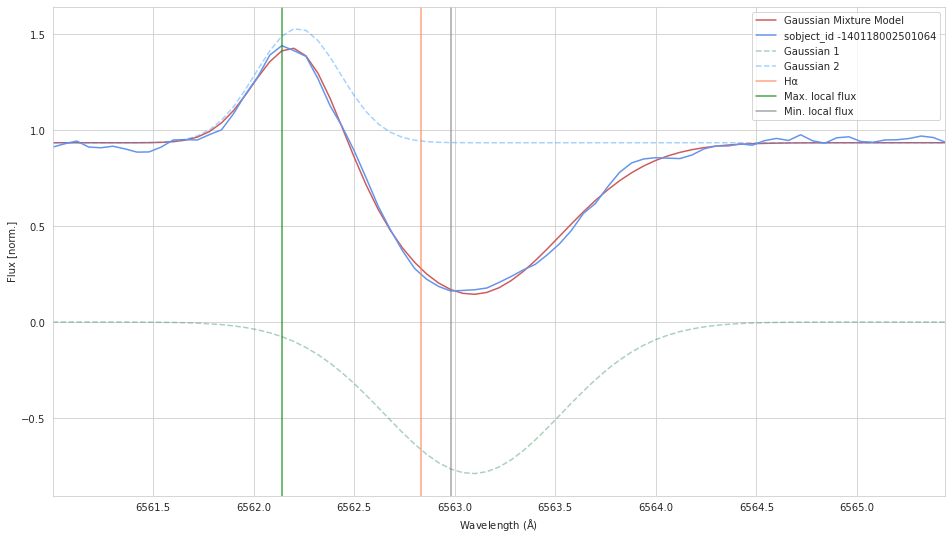
\includegraphics[scale=0.45]{figures/inverse p cygni 1.png}
\caption{A Gaussian mixture model fit of one of the identified inverse P Cygni spectrum. }
\end{figure}

\begin{figure}[!htb]
\centering
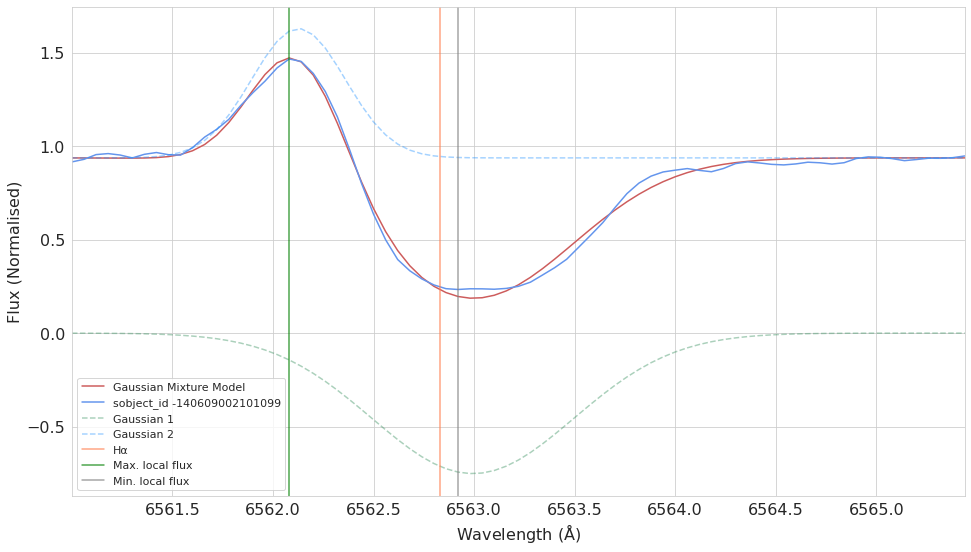
\includegraphics[scale=0.45]{figures/inverse p cygni fitted 2.png}
\caption{A Gaussian mixture model fit for sobject ID 140414005101301 (inverse P Cygni spectrum). }
\end{figure}

\section{Concluding Remarks}

Once the framework was in place, the sample data provided by Čotar et al. significantly accelerated the development of the methods discussed above. The primary reason for this is that methods can be tested and iterated at a more rapid pace given that the sample size was significantly smaller than GALAH DR3. Additionally, the sample data was well pruned and presumably only consisted of emission-line spectra although this may not be guaranteed. These conclusions make a strong case for the availability of open access data and code in addition to publications in astronomy. 

Dynamic time warping and indeed dynamic \emph{wavelength} warping was able to learn from the data presented and sufficiently generalise to provide pairwise distances that are able to capture the morphologies of the spectra. Combined with agglomerative hierarchical clustering, DTW can form the basis of a machine learning method that can identify, cluster and classify P Cygni, inverse P Cygni and other emission-line spectra.

Compared to methods such as k-means, logistic regression and t-SNE presented in Chapter 2, it can be argued that DTW is more sensitive to the morphological differences and similarities between spectra. t-SNE in particular is a well understood method that has been used to classify various classes of spectra from the GALAH survey. In Chapter 2 it was introduced that t-SNE can be used to identify H$\upalpha$ emission-line spectra in GALAH. Given the efficacy of DTW on a set of emission-line spectra provided by Čotar et al. this work considered whether t-SNE can be used as a pre-processing step in identifying emission-line stars prior to applying DTW. This hypothesis was tested during this work and the results are presented in the next chapter. 








